\documentclass[a4paper,11pt]{article}
\usepackage{algorithm}
\usepackage{algorithmic}
\usepackage[utf8]{inputenc}
\usepackage[total={6in, 9in}]{geometry}
\usepackage{hyperref}
\usepackage{amsthm, amssymb, amsmath,mathtools}
\usepackage{color}
\usepackage{diagbox}
\usepackage[usenames,dvipsnames]{xcolor}
\usepackage[T1]{fontenc}
\usepackage[scaled]{beramono}
\usepackage{listings}
\usepackage{subcaption}
\DeclareMathOperator{\E}{\mathbb{E}}

\definecolor{norah}{rgb}{1, 0, 0}
\definecolor{qiaoyi}{rgb}{0, 1, 0}
\definecolor{george}{rgb}{0, 0, 1}

\definecolor{dkgreen}{rgb}{0,0.6,0}
\definecolor{gray}{rgb}{0.5,0.5,0.5}
\definecolor{mauve}{rgb}{0.58,0,0.82}

\lstset{frame=tb,
  language=Python,
  aboveskip=3mm,
  belowskip=3mm,
  showstringspaces=false,
  columns=flexible,
  basicstyle={\small\ttfamily},
  numbers=none,
  numberstyle=\tiny\color{gray},
  keywordstyle=\color{blue},
  commentstyle=\color{dkgreen},
  stringstyle=\color{mauve},
  breaklines=true,
  breakatwhitespace=true,
  tabsize=3
}

\title{CS 590 Final Report: \\ PBFT Protocol Analysis with Game Theory and Multi-Agent Reinforcement Learning}
\author{Qiaoyi Fang, George Wang, and Norah Tan}
\date{April 23, 2021}


\begin{document}

\maketitle

\begin{abstract}
In distributed systems, consensus protocols such as PBFT are designed to achieve system reliability in the presence of of less than $f+1$ faulty nodes. We propose an attribution game to model the dynamics of offense and defense when the number of faulty nodes exceeds the safety threshold: while an attacker coordinates malicious nodes to breach consensus, an identifier aims to attribute the high-risk malicious nodes before violation. In this report, we present two approaches, namely, game theory and multi-agent reinforcement learning, to understand this complex game.
    
Our code is available at \href{https://github.com/georgezywang/BFT-RFForensics}{https://github.com/georgezywang/BFT-RFForensics}.
    
% - Explain the problem statement. What are you trying to achieve?\\
% - Explain your approach, and why other approaches do not work/shortcomings with them.\\
% - Explain the experiments and results.\\
% - Implementation code\\
% - What are your learnings? How would you go about extending this in the future?\\

\end{abstract}

\tableofcontents

\section{Introduction}\label{sec:intro}
% The adopted consensus protocol needs to satisfy the demands of specific application scenario regarding different distribution systems. 
% In the context of blockchain, all nodes maintain a public distributed data-ledger by consensus in a Peer-to-Peer (P2P) network, where there is only one canonical chain that all honest nodes will agree on and honest nodes are always able to add new blocks to the blockchain. The former property is known as \emph{safety} and the later is \emph{liveness}. 


In distributed systems, consensus protocols are designed to achieve overall system reliability -- that a set of honest nodes are capable of reaching agreements despite the presence of faulty nodes. In the context of \emph{state machine replication (SMR)}, the goal of a consensus protocol is to provide a fault-tolerant client-server interface by replicating servers and coordinating client interactions with server replicas, even when some of which are Byzantine faulty. Such protocols are called Byzantine Fault Tolerant (BFT) protocols.

A secure realization of SMR requires two guarantees that any two honest replicas cannot output different sequences of values and a value sent by a client will eventually be output by honest replicas \cite{sheng2021bft}. The former property is known as \emph{safety} and the later is \emph{liveness}. The honest replicas always follow the protocol exactly, whereas the Byzantines replicas may launch arbitrary attacks to maximize their own interests or simply to harm the entire distributed system \cite{Survey}.

Theoretically, there exists a maximum number of faults for obtaining agreement and termination, i.e., if the number of faults exceed it, the security could be violated. We then become interested in understanding the dynamics when the malicious replicas exceed the safety threshold and the potential defense mechanisms. More specifically, we hope to understand how to identify them through limited transcript monitoring and predict their response to the utilities of breaching consensus and the penalties of getting attributed. Existing literature aims to make faulty replicas accountable after consensus is breached \cite{sheng2021bft}. For more practical purposes, we would hope to identify the high-risk faulty ones before the occurrence of breaching consensus, without necessarily having any cryptographic irrefutable proof.

In this paper, we propose an attribution game to model the interplay of offense and defense in PBFT protocol when the number of faulty nodes exceeds the safety guarantees $f+1$. In the attribution game, two rational players, attacker and identifier, are motivated by opposite objectives. While the identifier hopes to identify high-risk malicious nodes to prevent consensus violation, the attacker aims to breach consensus while remaining undetected.

To analyze the attribution game, we presented two approaches, namely game theory and multi-agent reinforcement learning (MARL).
% {\color{george} summarize the approaches of game theory} 
We formulate the problem as an attacker-identifier game, which the attacker is a coordinated adversary and the identifier has access to limited number of logs. Both parties' objectives are to maximize their rewards given in a reward table. The game is played in a zero-sum setting.

To understand the attribution game with MARL, we reformulate the game as a decentralized variable order hidden markov process, the decentralized and partial observable properties of which lead to integrate the paradigm of centralized critic and decentralized actor with recurrent neural network encoder. After implementing the MARL algorithms and PBFT simulator, we study the simulation results.

The rest of the report is organized as follows.
In Section \ref{sec:bg}, we introduce the background of our project with more details, which includes PBFT protocols, game theory, and MARL.
In Section \ref{sec:related-work}, we discuss the related work.
In Section \ref{sec:idea}, we explain our idea and how the PBFT protocol is incorporated into our MARL setting. We also justify why MARL is a good candidate to analyze complex game dynamics.
In Section \ref{sec:game_analysis}, we apply game theoretic analysis to some simple scenarios in order to provide a theoretical support for MARL.
In Section \ref{sec:marl_approach}, we formalize the attribution game with MARL, describing the game model, algorithm, implementation, and experiments.
In Section \ref{sec:future}, we conclude this report and share our prospects on future directions and works.


\section{Background}\label{sec:bg}
\subsection{PBFT Protocols}\label{sec:pbft}
PBFT is a classical partially synchronous consensus protocol \cite{medium-2019}. It can tolerate up to $\frac13$ of the non-leader replicas acting malicious (more precisely, PBFT provides an optimal resilience of $t$ Byzantine faults out of $3t+1$ replicas). On a higher level, %{\color{norah}if we assume that all micro cryptographic level of security is established,}% 
the PBFT protocol proceeds in a sequence of consecutive views as follows, where each view has a unique primary replica and other nodes are called secondary replicas: 
\begin{itemize}
    \item \textbf{Request}: The client sends transactions to the primary replica.  
    \item \textbf{Pre-prepare}: The primary replica proposes a \textsc{PrePrepare} message containing transactions and broadcasts it to all replicas. When the replicas receive it, they will first verify it. If it is valid, they will add it to their respective transcripts and move on to the Preparing phase. 
    \item \textbf{Prepare}: Each secondary replica will broadcast a \textsc{Prepare} message that matches the accepted \textsc{PrePrepare} message. Each replica will then add its own \textsc{Prepare} to its transcript, accept \textsc{Prepare} messages from other nodes and add them to its transcript. Once a replica has $2t+1$ \textsc{Prepare} messages in its transcript that match the accepted \textsc{PrePrepare}, it will move on to the Committing phase.
    \item \textbf{Commit}: Similar to the Preparing phase, each replica broadcasts a \textsc{Commit} message to all replicas in the network, wait until there are $2t+1$ \textsc{Commit} messages in their transcripts, and then move on to the Replying phase. The only major difference between the Preparing and Committing phases is that in the Committing phase, the primary replica is allowed to broadcast a message.
    % \item \textbf{Prepare}: Upon receiving the \texttt{NewView} message, a replica will first verify it. If it succeeds, it will send a \texttt{Prepare} message to the leader. If the verification fails, then the replica will do nothing. This is the first round of voting. The leader then collects $\frac23$ such votes to form an aggregate signature \texttt{prepareQC} and sends it to all other replicas. 
    % \item \textbf{Commit}: Upon receiving \texttt{prepareQC} from the leader, a replica will now send a \texttt{Commit} message to the leader. This is the second round of voting. The leader then collects $\frac23$ such votes to form an aggregate signature \texttt{commitQC} and sends it to all other replicas.
    \item \textbf{Reply}: Each replica will inform the client of the matching \textsc{PrePrepare}, $2t+1$ \textsc{Prepare} messages, and $2t+1$ \textsc{Commit} messages. The client will see the results of the consensus. 
\end{itemize}
On the other hand, if the primary replica fails, a subroutine called \textbf{view-change} will be carried out and the system will designate a new primary replica. On a high level, when replicas see no new progress after some time, they broadcast a \textsc{ViewChange} message indicating that they want to advance to the next view. The view-change begin when $2t+1$ \textsc{ViewChange} messages from replicas are collected. 

\subsection{Game theory}\label{sec:gametheory}
Game theory is the study of mathematical models of strategic interaction among rational decision-makers, who strike to maximize their payoffs in the game. The attribution in consensus protocols can be considered as non-cooperative games. The analysis of a non-cooperative game usually focuses on predicting individual players' actions (strategies) and payoffs (utility for monetary values), and studying the Nash equilibrium. In a Nash equilibrium, each player is assumed to know the equilibrium strategies of the other players and no player has anything to gain by changing only their own strategy. 

We now formalize the description for a Nash equilibrium \cite{Nash-def}. Let $S_i$ be the set of all possible strategies for player $i$, where $i\in{1, \cdots, N}$. Let $s^* = (s^*_i, s^*_{-i})$ be a strategy profile, a set consisting of one strategy for each player, where $s^*_{-i}$ denotes the $N-1$ strategies of all the players except $i$. Let $u_i(s_i, s^*_{-i})$ be player $i$'s payoff as a function of the strategies. Then, the strategy profile $s^*$ is a Nash equilibrium if 
\begin{align}
    u_i(s^*_i, s^*_{-i}) \geq u_i(s_i, s^*_{-i}) \text{ for all }s_i\in S_i.
\end{align}
    
\subsection{Multi-agent Reinforcement Learning}\label{sec:marl}
Reinforcement learning (RL) is concerned with how intelligent agents maximize the long-term cumulative reward during the sequential interactions with the environment, the process of which is usually modelled by a Markov Decision process (MDP). Multi-agent Reinforcement Learning corresponds to the learning problem in which multiple agents learn simultaneously. 

We now formalize our description \cite{yang2021overview}. Through a trial-and-error procedure, each agent is trying to solve a MDP, which consists of a tuple of key elements
\begin{align}
    ( S, A, P, R, \gamma )
\end{align}
where
\begin{itemize}
    \item $S$ is the set of environmental states.
    \item $A$ is the set of agent's possible actions.
    \item $P:S\times A\to \Delta(S)$ is the transition probability from a state $s\in S$ in timestep $t\in\mathbb{N}$ to the state $s'\in\mathbb{S}$ in the next timestep, given the agent's action $a\in A$.
    \item $R:S\times A\times S\to\mathbb{R}$ is the reward function that returns a scalar value to the agent as a result of the transition from $s$ to $s'$ under action $a$.
    \item $\gamma\in[0,1]$ is the discount factor that represents the value of time.
\end{itemize}

In MARL, the transition of the environment states and the reward function for each agent is determined by all agents' joint actions. Therefore, the decision-making process that involves multiple agents is usually modelled through the multi-player extension to the Markov decision process: a stochastic game described by
\begin{align}
    (N, S, \{{\bf{A_i}}\}_{i\in{1, \cdots, N}}, P,  \{\bf{R_i}\}_{i\in{1, \cdots, N}}, \gamma ),
\end{align}
where
\begin{itemize}
    \item $N\geq 2$ is the number of agents.
    \item $S$ is the set of environmental states shared by all agents.
    \item $\bf{A_i}$ is the set of actions of agent $i$.
    \item $P:S\times {\bf{A_1}}\times \cdots\times {\bf{A_N}} \to\Delta(S)$ is the transition probability from a state $s\in S$ in timestep $t\in\mathbb{N}$ to the state $s'\in S$ in the next timestep, given the agents' joint action ${\bf{a}}\in {\bf{A_1}}\times \cdots\times \bf{A^N}$.
    \item ${\bf{R_i}}:S\times {\bf{A_1}}\times \cdots\times {\bf{A_N}}\times S\to\mathbb{R}$ is the reward function that returns a scalar value to agent $i$ as a result of the transition from $s$ to $s'$ under action $\bf{a}$.
    \item $\gamma\in[0,1]$ is the discount factor that represents the value of time.
\end{itemize}

\section{Related Work}\label{sec:related-work}
% PBFT attribution
\paragraph{PBFT attribution.} A recent work on BFT protocols is brought to our attention. Sheng \emph{et al.} \cite{sheng2021bft} mathematically formalized the study of a forensic support for BFT protocols such that after a security breach, we can identify as many of the malicious replicas who participated in the attack as possible. The identification of malicious replicas is the form of an irrefutable cryptographic proof of culpability and is conducted as distributedly as possible. The paper \cite{sheng2021bft} focused on three popular BFT protocols to characterize the forensic support, which include PBFT, the first practical BFT SMR protocol in the partially synchronous setting. %{\color{norah}Add one sentence why we are interested in PBFT.} 

% game theory on consensus
\paragraph{Game theory on consensus protocols.} While reading the literature, we notice that there are several researches on applying game theory concepts to the design and analysis of consensus algorithms, which serve as a baseline of analyzing consensus protocols \cite{10.5555/1296179}. Liu \emph{et al.} \cite{Survey} provided a detailed summary on game theory as an analytic tool in blockchain. There also exists previous works on applying game theoretic analysis to some specific protocols, or creating novel protocols that possess desirable properties of Nash Equilibrium, i.e. when reaching the Nash equilibrium, entities will not be able to increase their gains by being malicious. Some other examples include but without limiting to the following:
\begin{itemize}
    \item In \cite{Kiayias-CRYPTO2017}, Kiayias \emph{et al.} presented a game theoretic incentive mechanism in order to encourage active participation in Ouroboros--a proof-of-stake (PoS) blockchain protocol--by allowing such honest behaviors to have the highest possible payoff. Even though it may not be directly applicable to other PoS protocols, the idea of regulating practical behaviors to fit theoretical assumptions is helpful.
    \item In \cite{Alzahrani-DGTS2018}, Alzaharni \emph{et al.} presented an enhanced protocol based on Tendermint by introducing randomness. They used game theory as a tool to prove its effectiveness and robust security performance such that it is ensured that rational entities should always behave honestly.
\end{itemize}

\paragraph{MARL on consensus protocols.}
%- recent paper demonstrates the potential, yet lack of attention, lack of attention of combining RL with bc
% http://shura.shu.ac.uk/27490/2/AI_for_Energy_Market%20accepted.pdf
The paper \cite{Jogunola-ieee2021} by Jogunola \emph{et al.} reviewed consensus algorithms and deep RL in energy trading systems (ETS) as well as their principles, models, active research efforts and unresolved challenges.
It demonstrated to us the potential of combining block chain with artificial intelligence (AI) to realize secured and intelligent ETS. Despite the immutability of transaction records, the central idea is to forecast and address data analytic related issues using AI algorithms, as the distributed consensus protocols generate deluge of data.  

The review also pointed out that regardless of the current interest in consensus protocols and RL respectively, little effort has been made at jointly exploiting them. They argued that new insights are actively required to harness the full potentials of consensus protocols and RL.



\section{Attribution Game}\label{sec:idea}
One important feature in the forensic support of BFT protocols \cite{sheng2021bft} is the use of transcripts from honest parties as input. We are thus inspired to ask the question: when \textbf{combining game theoretic models with transcripts analysis}, can we obtain a better understanding of the strategic interaction between the attackers, honest decision-makers, or some other parties in the protocols? More specifically, will we be capable of identifying or predicting Byzantine replicas during the execution of the protocol, instead of after the security breaches happen? Or to be furthermore specific, we would like to understand:
\begin{itemize}
    \item From the identifier's point of view, what is the minimal number of transcripts that we need in order to detect malicious replicas and prevent a consensus violation?
    \item From the attacker's point of view, under different reward structures (explained more in Section \ref{sec:game_analysis}, how will the attacker change its strategies?
\end{itemize}
To model the full dynamics of such offense and defense in PBFT protocol when the number of faulty nodes exceeds $f+1$, we propose the attribution game, consisting of two rational players, the attacker and identifier.
The attacker has full control over $k \geq f+1$ malicious nodes in the system, while the identifier has access to the transcripts of $m$ randomly assigned nodes. The identifier hopes to identify high-risk malicious nodes to prevent consensus violation, while the attacker aims to breach consensus while remaining undetected. To address the two proposed questions with the attribution game, we utilized game theory and multi-agent reinforcement learning to study the game.






%Some game-theory based algorithms, for instance, \emph{multi-agent reinforcement learning (MARL)}, seem promising in offering the insights we want. 
% {\color{norah}Two more sentences about MARL, maybe ideas used in our project.} 
% {\color{norah}Put our Results here. } 
% {\color{norah}It will be a good idea to compare BFT forensics with our model somewhere in the report.} 
% -  PBFT
%  - attacks on PBFT
%  - understand game theoretic dynamics
% 	- identifier can access to transcript, - makes RL a good candidate to analyze complex games
% 	- tune rewards
% 		- (high/low concensus breanched payoff + low/high caught penality) attacker's strategy (number of malicious nodes/total nodes, ...)
% 		- (identifier access to number transcripts from replicas) - what's the minimal number of transcripts we need to detect malicious replicas and prevent a consensus violation  - pbft forensics paper


% Our project is motivated by the situations where 
% - an aggregate attacker in charge of multiple malicious nodes $>f+1$
% - an identifier that monitor transcripts of any k nodes. 
%     - During and after the execution, each replica keeps all received messages as transcripts in order to prevent malicious nodes to provide counterfeit evidence.
    
% In conventional game theory formation, \\
%     - rational players\\
%     - identifier' reward structures\\
%     - attacker' reward structures\\

% The game is difficult to solve\\
%     - huge action space leads to strategies profiles\\
%     - players have access to history\\




%\section{Methodology}\label{sec:methodology}
%\subsection{Attacker and Identifier}
%\subsection{Rewards and Penalties}
%(high/low concensus breanched payoff + low/high caught penality)


%- Explain your approach, and why other approaches do not work/shortcomings with them.
% 	- related work(pbft forensics, ...)
%	- MultiAgent RL
%		- paper
\section{Game Theoretic Analysis on Attribution Game}\label{sec:game_analysis}
To provide a theoretical support for the MARL model, we apply game theoretic analysis to some simple scenarios and provide justifications for a Nash Equilibrium in this scenario. Throughout the analysis, we use the notation in Table~\ref{tab:Notations}. Though in the MARL implementation, we set \(e_m\) to \(1\) for the interest of model convergence.

\begin{table}[h!]
    \centering
     \begin{tabular}{||c c c||} 
     \hline
     Hyperparameter & Definition & Value Used \\ [0.5ex] 
     \hline\hline
     \(m\) & number of logs the identifier has access to & 1\\
     \(\alpha_i\) & identifier reward if consensus reached & 0  \\ 
     \(\alpha_m\) & attacker reward if consensus reached & 0 \\
     \(\beta_i\) & identifier reward if consensus breached & -5\\
     \(\beta_m\) & attacker reward if consensus breached & 5 \\
     \(d_i\) & identifier reward if correct detection & 3 \\ 
     \(d_m\) & attacker reward if correct detection & -3 \\ 
     \(e_i\) & identifier reward if incorrect detection & -3 \\ 
     \(e_m\) & attacker reward if incorrect detection & 3 \\ 
     [1ex] 
     \hline
     \end{tabular}
     \caption{Notations and Definitions}
     \label{tab:Notations}
\end{table}

\subsection{Analysis Setup}
Given a system with \(4\) nodes, \(2\) of which are Byzantine, we formalize a simple double voting attack. Assume the leader \(l\) and an arbitrary node \(n_1\) is Byzantine while \(n_2\), \(n_3\) are functioning properly. We analyze the log before the commit phase, which any succeeding event will directly indicate whether consensus is breached. Note that a game theoretic analysis model would be combinatorial with respect to the number of nodes whose scripts are retrieved by the identifier. Therefore, for simplicity, we would use game theoretic analysis to analyze a simple case of \(m = 1\) where \(m\) is the number of logs that the identifier gets to access, with the same settings as mentioned. By the quorum intersection argument, the identifier can identify at most \(t + 1\) faulty nodes even after consensus is breached, and that a forensic support only works when \(d \leq t + 1\) so we would assume the identifier would try to identify at most \(2\) malicious nodes.
Therefore, there are total of \(\binom{4}{0} + \binom{4}{1} + \binom{4}{2}= 11\) possibilities of identifier's strategy for each log it reads. There are \(4\) possible logs that the identifier may read, so there are in total \(4 \times 11 = 44\) strategies we would need to analyze.


\subsection{Strategy Payoffs}
For this game, we first discuss the strategy of the malicious party, which we assume can be coordinated. 

\textbf{NOOP Strategy:} The simplest strategy is to not cheat, and hence the payoff table should be the same for the identifier regardless of which log it reads. The rewards of each strategy that the identifier could take are summarized in Table~\ref{tab:NotCheatPO1} and Table~\ref{tab:NotCheatPO2}. For the interest of space, we would assume \(\alpha_i = \alpha_m = 0\).

\begin{table}[!htb]
    \centering
    \begin{tabular}{|l||*{5}{c|}}\hline
        \backslashbox[12em]{Attacker}{Identifier}
        &\makebox[4em]{None}&\makebox[4em]{\(n_1\)}&\makebox[4em]{\(n_2\)}
        &\makebox[4em]{\(n_3\)}&\makebox[4em]{\(l\)}\\\hline\hline
        Not Cheat & \(\alpha_m \mid \alpha_i\) & \(d_m \mid d_i\) & \(e_m \mid e_i\) & \(e_m \mid e_i\)  & \(d_m \mid d_i\) \\\hline
    \end{tabular} 
    \caption{Payoff Table for Identifier identifying \(\leq 1\) malicious node}
    \label{tab:NotCheatPO1}
\end{table}

\begin{table}[!htb]
    \centering
    \begin{tabular}{|l||*{6}{c|}}\hline
        \backslashbox{Attacker}{Identifier}
        &\makebox[4em]{\(l\) and \(n_1\)}&\makebox[16em]{an \(i \in \{l, n_1\}\) and a \(j \in \{n_2, n_3\}\)}&
        \makebox[4em]{\(n_2\) and \(n_3\)}\\
        \hline\hline
        Not Cheat & \(2d_m \mid 2d_i\) & \(d_m + e_m \mid d_i + e_i\) & \(2e_m \mid 2e_i\)\\\hline
    \end{tabular} 
    \caption{Payoff Table for Identifier identifying \(2\) malicious node}
    \label{tab:NotCheatPO2}
\end{table}

\textbf{Double Vote Strategy:} We then consider the case in which the malicious nodes choose to cheat, and initiate a double vote attack to the system. To break consensus, the leader sends a proposal \(v\) to \(n_1\), \(n_2\), and \(v'\) to \(n_1\), \(n_3\). We stick to analyzing the payoffs before the commit phase, when the identifier needs to decide what strategy to take. In this case, the identifier's strategy should be dependent on which log it reads.
Assuming all messages are signed, when reading the log of \(n_1, n_2, n_3\), the identifier should figure that the leader was sending conflicting messages given that all honest nodes have been broadcasting the messages they received. Therefore, the identifier's strategy would be choosing among only reporting \(l\), or reporting \(l\) and an additional node. However, only reporting \(l\) would still result in a consensus breach per our definition. The payoff table for this case is hence formulated as inume \(\alpha_i = \alpha_m = 0\).
 Table~\ref{tab:DoubleVotePO1}.
\begin{table}[!htb]
    \centering
    \begin{tabular}{|l||*{3}{c|}}\hline
        \backslashbox{Attacker}{Identifier}
        &\makebox[5em]{\(l\)}&\makebox[10em]{\(l\) and a \(j \in \{n_2, n_3\}\)}&
        \makebox[5em]{\(l\) and \(n_1\)}\\
        \hline\hline
        Double Vote & \(\beta_m + d_m \mid \beta_i + d_i\) & \(\beta_m + d_m + e_i \mid \beta_i + d_i + e_i\) & \(2d_m \mid 2d_i\)\\\hline
    \end{tabular} 
    \caption{Payoff for Identifier for Double Voting Attack and Reading Any of \(n_1, n_2, n_3\)'s Log}
    \label{tab:DoubleVotePO1}
\end{table}

We now consider the case which the identifier reads the leader's log. The leader should have received two \textsc{Prepare} messages from \(n_1\), for both \(v\) and \(v'\), which implies that \(n_1\) is malicious. Therefore, we can formulate the payoff as in Table~\ref{tab:DoubleVotePO2}.

\begin{table}[!htb]
    \centering
    \begin{tabular}{|l||*{3}{c|}}\hline
        \backslashbox{Attacker}{Identifier}
        &\makebox[5em]{\(n_1\)}&\makebox[10em]{\(n_1\) and a \(j \in \{n_2, n_3\}\)}&
        \makebox[5em]{\(l\) and \(n_1\)}\\
        \hline\hline
        Double Vote & \(\beta_m + d_m \mid \beta_i + d_i\) & \(\beta_m + d_m + e_i \mid \beta_i + d_i + e_i\) & \(2d_m \mid 2d_i\)\\\hline
    \end{tabular} 
    \caption{Payoff for Identifier for Double Voting Attack and Reading Any of \(l\)'s Log}
    \label{tab:DoubleVotePO2}
\end{table}
% assume the messages are all signed
% then reading the log for n_1, n_2, n_3 will all reveal that the leader was sending conflicting messages \implies leader is faulty
% reading the log fo leader implies n_1 is faulty since it receives two conflicting votes from n_1

\textbf{Overturning Block Strategy:} We finally consider a more sophisticated approach of attacking, which the adversary tries to overturn an existing block. This can be done with the following procedure: in some view \(e\), a replica outputs \(CommitQC\) formed with \textsc{Commit} from \(l, n_1, n_2\) and hence hold lock on \((v, e)\). \(n_3\) holds a lower lock for a different value. The system remains as such for several views, with no higher lock being formed. Then at some view \(e^*\), the leader receives locks from \(l, n_1, n_3\) and hence proposes \(v'\). This makes \(n_2, n_3\) both unlock and vote for \(v'\), and overturns \(v\) in some later view \(e'\). This attack is achieved by the faulty replicas maliciously sending lower locks, and the identifier shall identify the malicious nodes based on such information. Since the honest nodes broadcasts the messages they receive, if the identifier gets to read any of the non-leader's log, it should notice the malicious leader, and hence the payoff table can be formulated as Table~\ref{tab:OverturnL}. Observe that this is very similar to the double voting attack.

\begin{table}[!htb]
    \centering
    \begin{tabular}{|l||*{3}{c|}}\hline
        \backslashbox{Attacker}{Identifier}
        &\makebox[5em]{\(l\)}&\makebox[10em]{\(l\) and a \(j \in \{n_2, n_3\}\)}&
        \makebox[5em]{\(l\) and \(n_1\)}\\
        \hline\hline
        Overturn & \(\beta_m + d_m \mid \beta_i + d_i\) & \(\beta_m + d_m + e_i \mid \beta_i + d_i + e_i\) & \(2d_m \mid 2d_i\)\\\hline
    \end{tabular} 
    \caption{Payoff for Identifier for Overturn Attack and Reading Any of \(n_1, n_2, n_3\)'s Log}
    \label{tab:OverturnL}
\end{table}

If the identifier reads the leader's log, then it should discover that \(n_1\) has maliciously voted for a lower lock, and we can hence formulate the payoff table as Table~\ref{tab:OverturnN}.

\begin{table}[!htb]
    \centering
    \begin{tabular}{|l||*{3}{c|}}\hline
        \backslashbox{Attacker}{Identifier}
        &\makebox[5em]{\(n_1\)}&\makebox[10em]{\(n_1\) and a \(j \in \{n_2, n_3\}\)}&
        \makebox[5em]{\(l\) and \(n_1\)}\\
        \hline\hline
        Overturn & \(\beta_m + d_m \mid \beta_i + d_i\) & \(\beta_m + d_m + e_i \mid \beta_i + d_i + e_i\) & \(2d_m \mid 2d_i\)\\\hline
    \end{tabular} 
    \caption{Payoff for Identifier for Overturn Attack and Reading Any of \(l\)'s Log}
    \label{tab:OverturnN}
\end{table}

Were the attackers choose to launch any nontrivial attacking strategy, the identifier will be able to identify some if not all malicious nodes. However, it is not obligated to play such strategy, and that it can choose to. For any attacking strategy that the attacker initiates, the identifier could also try to identify none, or only one node, while suffering the reward of consensus being breached. This can be formulated as Table~\ref{tab:TVNV}. There are more possibilities of the identifier not identifying the malicious node that is proven to be faulty using the logs. This can be formulated in a similar manner, and thus we will not list more tables here. 

\begin{table}[!htb]
    \centering
    \begin{tabular}{|l||*{4}{c|}}\hline
        \backslashbox[8em]{Attacker}{Identifier}
        &\makebox[4em]{None}&\makebox[4em]{\(n_1\)}&\makebox[4em]{\(n_2\)}
        &\makebox[4em]{\(n_3\)}\\\hline\hline
        Attack & \(\beta_m \mid \beta_i\) & \(\beta_m + d_m \mid \beta_i + d_i\) & \(\beta_m + e_m \mid \beta_i + e_i\) & \(\beta_m + e_m \mid \beta_i + e_i\) \\\hline
    \end{tabular} 
    \caption{Payoff Table for Trivial Identifier with Nontrivial Attacker}
    \label{tab:TVNV}
\end{table}

\subsection{Nash Equilibrium Formulation}
Though we have simplified the model as best as we can, taking all strategies into account is still extremely complicated, so we would like to provide a simple example, which the attacker would only choose among two strategies: \textit{NOOP} or \textit{Double Vote}, with probability \(p\), \(1 - p\) respectively. We further assume that the identifier only reads the leader's log, but the identifier has access to all \(11\) corresponding strategies. We order the strategies using the canonical order presented in the tables, each with probability \(b_1, b_2, \dots, b_{10}, 1 - \sum_{i = 1}^{10} b_i\). We then analyze the payoff of each party's strategies. 

If the attacker choose to play not cheat, then the expected payoff would be
\begin{align*}
    \mathbb{E}\left[A_{NOOP} \right] &= b_1\alpha_m + b_2(d_m + \alpha_m) + (b_3 + b_4)(e_m + \alpha_m) + b_5(d_m + \alpha_m) \\
    &\ \ \  + 2b_6(d_m + \alpha_m) + (d_m + e_m + \alpha_m)(b_7 + b_8 + b_9 + b_10) + (1 - \sum_{i = 1}^{10} b_i)(e_m + \alpha_m)
\end{align*}
Similarly, the expected payoff for using the double voting strategy would be 
\begin{align*}
    \mathbb{E}\left[A_{\textsc{DoubleVote}} \right] &= b_1\beta_m + (b_2 + b_5)(\beta_m + d_m) + (b_3 + b_4)(\beta_m + e_m) \\
    &\ \ \ + b_6(\alpha_m + 2d_m) + (b_7 + b_8 + b_9 + b_{10}) + (1 - \sum_{i = 1}^{10} b_i)(e_m + \beta_m)
\end{align*}
We now consider the strategies of the identifier and it's payoff.
\begin{align*}
    &\mathbb{E}\left[I_{None}\right] = p\alpha_i + (1 - p)\beta_i\\
    &\mathbb{E}\left[I_{l}\right] = (d_i + \alpha_i)p + (\beta_i + d_i)(1 - p)\\
    &\mathbb{E}\left[I_{n_1}\right] = (d_i + \alpha_i)p + (\beta_i + d_i)(1 - p)\\
    &\mathbb{E}\left[I_{n_2}\right] = (e_i + \alpha_i)p + (\beta_i + e_i)(1 - p)\\
    &\mathbb{E}\left[I_{n_3}\right] = (e_i + \alpha_i)p + (\beta_i + e_i)(1 - p)\\
    &\mathbb{E}\left[I_{l \& n_1}\right] = 2p(d_i + \alpha_i) + (1 - p)(2d_i + \alpha_i)\\
    &\mathbb{E}\left[I_{l \& n_2}\right] = \mathbb{E}\left[I_{l \& n_3}\right] = \mathbb{E}\left[I_{n_1 \& n_2}\right]\\ 
    &\ \ \ \ \ \ \ \ \ \ \ = \mathbb{E}\left[I_{n_1 \& n_3}\right] = p(d_i + e_i +\beta_i) + (1 - p)(2d_i + \alpha_i)\\
    &\mathbb{E}\left[I_{n_2 \& n_3}\right] = 2p(e_i + \alpha_i) + (1 - p)(2e_i + \beta_i)
\end{align*}
We can hence calculate the Nash Equilibrium using the preceding equations. 

\section{Approaching Attribution Game with MARL}\label{sec:marl_approach}
\subsection{Game Model}
In order to realistically capture the complexity of interactions in PBFT with MARL, we consider the attribution game to be modelled by a decentralized variable order hidden Markov model $V$, where the transition to the next state depends on a variable number of conditioning factors in the previous states and agents only have partial knowledge of the true state of the environment. In contrast to usual application of settings of Reinforcement Learning, attribution game has the variable order property because each replica maintains a log of events since the proposal of the genesis block that is used to determine the next behavior, and furthermore a successful attack can take place across multiple views \cite{sheng2021bft}. In addition, its property of partial observability is embedded in the central question of consensus protocols that address Byzantine failures.

Formally, we can state the model as
\begin{align}
    V = (I, p(s_0), S, {\bf{A}}, P,  R, \Omega, \gamma),
\end{align}
where $I$ is the set of agents in which agent $i \in \{\text{att}, \text{id}\}$. $\gamma \in [0,1)$ is the discount factor, $s \in S$ is the true state of the environment, and $p(s_0)$ is the probability distribution of initial state $s_0$ that describes the randomly chosen malicious node ids $M$ controlled by the attacker $att$ and the nodes ids $T$ monitored by the identifier $id$.

As we consider partially observable settings, two agents only have access to observation $o_i \in \Omega_i$ drawn according to their own observation function $O(s_t,i)$ where $i \in \{\text{att}, \text{id}\}$.
More specifically, the attacker agent's observation $o$ consists of the messages received by the malicious nodes $M$ at the timestep $t$, while the identifier receives the aggregate transcript of the monitored nodes $T$, i.e., the received messages of $T$. Both agents have a history
\begin{align}
    \tau_i \in T \vcentcolon= (\Omega_i \times {\bf{A_i}})^*.
\end{align}

At each timestep, each agent selects an action $\bf{a_i} \in \bf{A_i}$: $\mathbf{A_{\text{att}}}$ is the combination of messages with attributes such as message type, sequence number, and receiver id, therefore, $\bf{a_{\text{att}}}$ contains a list of message attributes, denoting as subactions $a'_{\text{att}}$; as $\bf{A_{\text{id}}}$ defines the set of actions for the identifier to identify the malicious nodes in the system, $\bf{a_{id}}$ contains the number of replicas of boolean subactions $a'_{\text{id}}$. The implementation of actions is discussed in Section \ref{sec:codes} in details. At timestep $t$, joint actions $\bf{a_t}$ together with the past sequence of states $\{s_0, ..., s_{t}\}$ lead to the next state $s_{t+1}$ according to the transition function $P(s_{t+1}|\mathbf{a_t}, s_{t}, ..., s_0)$ with agent $i$ receiving reward $r_i$ = $R_i(s_{t}, ..., s_0,\bf{a})$. The agents learn separate policies $\pi_i$ that induces a joint action-value function


\begin{align}
    Q^{\pi}_{i}(s,{\bf{a}})=\E_{s_0 \sim p}\left[\sum_{t=0}^{\infty}\gamma^tr_t\Big\vert s_0, \bf{\pi}\right].
\end{align} 

\subsection{Algorithm}
\paragraph{Centralized Critic, Decentralized Actor.} In the hope of effectively learning policies for agents, we adapted the paradigm of centralized training with decentralized execution (CCDA) \cite{SIMOES202040}, meaning that learning data from agents are gathered collectively to optimize critic which provides better value evaluation of state-action pairs, while decentralized execution promises flexible adaptation to competitive games, including the attribution game. In addition to better state-action evaluation, the parameters sharing in centralization of critic could potentially boost the training efficiency of the learning algorithm, which is important in our problem as the actor policies $\pi$ for attacker and identifier cannot be jointly trained due to the lack of homogeneity between the two agents.\\

Adaptations were made on CCDA, particularly to modify the policy gradient theorem for multiple actions. As mentioned in 7.1, the required action space of agents are inherently combinatorial, with action input of each timestep effectively consisting of multiple discrete actions. In contrast to single action in the general problem formation of MARL, this particular distinction demands modifications in the central policy gradient theorem of CCDA. Parameterized with respect to $\theta$, policy $\pi({\bf{a}}|s, \theta)$ outputs multiple actions $\mathbf{a} = \{a_1, ..., a_k\}$. The expected cumulative reward function is defined as

\begin{equation}
\begin{split}
J(\theta) & = \sum_{s \in S} \mu(s) \sum_{\bf{a} \in \bf{A}}\pi(\mathbf{a}|s,\theta)Q_\pi(s, \mathbf{a})\\
& \approx \sum_{s \in S} \mu(s) \sum_{\mathbf{a} \in \mathbf{A}}\prod^k_{i=1}\pi(a_i|s,\theta) Q_\pi(s, \mathbf{a}),
\end{split}
\end{equation}
where $\mu(s)$ is the stationary on-policy state distribution.

To optimize policy $\pi({\bf{a}}|s, \theta)$, the gradient $\nabla_\theta J(\theta)$ can be computed as 
\begin{equation}
\begin{split}
\nabla_\theta J(\theta) & = \sum_{s \in S} \mu(s) \sum_{\bf{a} \in \bf{A}} \nabla_\theta \pi(\mathbf{a}|s,\theta)Q_\pi(s, \mathbf{a})\\
& \approx \sum_{s \in S} \mu(s) \sum_{\mathbf{a} \in \mathbf{A}}\nabla_\theta \prod^k_{i=1}\pi(a_i|s,\theta) Q_\pi(s,\mathbf{a})\\
& = \sum_{s \in S} \mu(s) \sum_{\mathbf{a} \in \mathbf{A}} \prod^k_{i=1}\pi(a_i|s,\theta) \left(\sum_{j=1}^{k}\frac{\nabla_\theta \pi(a_j|s,\theta)}{\pi(a_j|s,\theta)}\right)Q_\pi(s,\mathbf{a})\\
& = \E_{\pi_\theta}\left[\sum^k_{i=1}\ln\pi(a_i|s, \theta)Q_\pi(s,\mathbf{a})\right].
\end{split}
\end{equation}
The final expression of $\nabla_\theta J(\theta)$ is a quantity that can be sampled at each timestep, which yields the update:
\begin{equation}
    \theta_{t+1} \vcentcolon= \theta_{t} +  \alpha \sum^k_{i=1}\ln\pi(a_i|s, \theta)Q_\pi(s,\mathbf{a}),
\end{equation}
where $\alpha$ is the hyperparamter learning rate. In the implementation of equation (6), $s$ is extended to sequential input of observations $\bf{o}$. For the convenience of notations, we denote $\mathbf{s_t}$ as the sequence of state trajectory $\{s_0, ..., s_t\}$. Similarly, $\mathbf{o_t}$ denotes the sequence of observations $\{o_0, ..., o_t\}$.  

\begin{algorithm}
\caption{CCDA in the attribution game}
\begin{algorithmic}
\REQUIRE Attacker policy function $\pi_{att}(\bf{a}|\bf{o}, \theta_{att})$ with learning rate $\alpha_{att}$, identifier policy function $\pi_{id}(\bf{a}|\bf{o}, \theta_{id})$ with $\alpha_{id}$, and shared critic $Q(\bf{o}, \bf{a_{att}}, \bf{a_{id}}, \phi_{q})$ with $\alpha_{q}$

\STATE Initialize $s_0 \sim p(s_0)$, $\theta_{att}$, $\theta_{id}$, and $\phi_{q}$
\STATE Sample $\bf{a_{att}} \sim \pi_{\theta_{att}}$ and $\bf{a_{id}} \sim \pi_{\theta_{id}}$ where $\bf{a} = {a_{att}, a_{id}}$.
%balance the 
\WHILE{not done}
    \STATE Sample $\bf{r} \sim R(\bf{s}, \bf{a})$ where $\mathbf{r} = \{r_{arr}, r_{id}\}$
    \STATE Sample next state $s' \sim P(s'|\bf{s}, \bf{a})$ and $o'_{att}$, $o'_{id}$ from $O(s')$
    \STATE Then sample $\bf{a_{att}} \sim \pi_(\bf{o'_{att}},\theta_{att})$ and $\bf{a_{id}} \sim \pi_(\bf{o'_{id}}, \theta_{id})$
    \STATE Update attacker policy parameters:\\ $\theta_{att} \leftarrow \theta_{att} + \alpha_{att}Q_\pi(\bf{o},\mathbf{a})\sum_{a \in \mathbf{a_{att}}}\ln\pi(a_{att}|\mathbf{o_{att}}, \theta_{att})$ 
    \STATE Similarly, update identifier policy parameters: \\ $\theta_{id} \leftarrow \theta_{id} + \alpha_{id}Q_\pi(\bf{o},\mathbf{a})\sum_{a \in \mathbf{a_{id}}}\ln\pi(a_{id}|\mathbf{o_{id}}, \theta_{id})$
    \STATE Compute the temporal difference error for critic at time $t$:\\ $\delta = \bf{r} + \gamma Q_\phi(\mathbf{s'}, \mathbf{a'}) - Q_\phi(\mathbf{s}, \mathbf{a})$
    \STATE Update critic parameters with the new correction:\\
    $\phi_{q} \leftarrow \phi_{q} + \alpha_{q}\delta Q_\phi(\mathbf{s}, \mathbf{a})$
    \STATE Update $a \leftarrow a'$ and $s \leftarrow s'$.
\ENDWHILE
\end{algorithmic}
\end{algorithm}
\paragraph{LSTM Encoder} \cite{lstm-Hochreiter} \cite{chu2019multiagent} \cite{sukhbaatar2016learning}
In addition to employing CCDA to deploy policy learning, we also utilized Long Short-Term Memory (LSTM) components to encode the sequential and temporal knowledge of the observation inputs to facilitate this process. An LSTM unit structure is a cell that consists of an input gate, an output fate and a forget date, regulating the information flow in the cell of entering, leaving, and staying. To counter the variable order and partial observability of the game, we leverage LSTM to enable the agents to selectively process and reason connections between observation data of different timesteps in the sequential input. 

\subsection{Implementation}\label{sec:codes}
To analyze dynamics of the attribution game under different settings, we developed a codebase that allows high flexibility of game configurations and easy setup. To achieve this goal, our code was encapsulated into four main modules:
\begin{itemize}
    \item an implementation of PBFT protocol including both normal and view change mode,
    \item a protocol simulator that functions as the interactive environment of the replicas and two agents,
    \item a MARL framework that implements the agents together with learner that updates the agent policies and critic from the sampled learning data,
    \item an experiment framework that automates the process of sampling episodes, training agents, logging and visualizing results.
\end{itemize}
All modules have been tested, and the results and discussions of our experiments will be included in Section \ref{sec:experiments} and \ref{sec:discussion}. In the following sections, we will discuss the four mentioned modules in detail.
\subsubsection{PBFT protocol}
The PBFT protocol module contains a simplified implementation of normal and view change modes of the protocol. To simulate a network of replica servers with signatures, we implemented a replica class that follows protocol behaviors to handle signed messages.
\paragraph{Messages.} For simplification, We had messages to be sent in a defined class and avoided the need of serialization and parsing. Furthermore, we assumed the attacker is incapable of forging counterfeit signatures, e.i. it can send messages only with sender $s \in$ malicious nodes $M$, and all messages are sent from members in the system; in this way, we also avoided to implement signature verification.
\begin{lstlisting}
// in protocols/PBFT/message.py
class PBFTMessage():
    def __init__(self, args, msg_type, view_num, seq_num, signer_id, val, receiver_id):
        self.args = args
        self.msg_type = type_dict[msg_type]
        self.view_num = view_num
        self.seq_num = seq_num
        self.signer_id = signer_id
        self.val = val
        self.receiver_id = receiver_id
        self.certificate = certificate  # if msg_type is PrepareCertificate, CommitCertificate or NewView
\end{lstlisting}    
A message in our PBFT protocol is in one of eleven types: 
\begin{lstlisting}
// in protocols/PBFT/message.py
type_dict = {
            "PrePrepare": 0,  
            # proposing a new block, sent by the primary only
            "Prepare": 1,     
            # broadcast in the preparing phase, sent by non-primary only
             "Commit": 2,      
             # broadcast in the commit phase
             "ViewChange": 3,  
             # sent when primary is suspected to be faulty
             "NewView": 4,     
             # sent by the new primary to initiate a new view
             "PrepareCertificate": 5, 
             # proves that 2f+1 nodes has agreeed to enter preparing phase
             "CommitCertificate": 6,  
             # proves that 2f+1 nodes has agreed to commit it
             "BlockCommit": 7,        
             # a node inform the simulator that it has committed
             "RequestClient": 8,      
             # the new primary asked to simulator to go to request with a provided sequence number
             "No-op": 9,
             # for the attacker agent to skip the action
             "Client": 10, 
             # simulator sent to the primary on a new block}
\end{lstlisting}
\paragraph{Information storage.} In addition to messages, we also implemented information storage for node to store a list of key information to represent its current state including:
\begin{itemize}
    \item list of its peers in the system
    \item current view number
    \item a log indexed by sequence number that records the block value, received signatures in the preparing and committing phases
    \item a view change log indexed by view number that records the received signatures in the view change phase
\end{itemize}
The above features guarantee the basic functionality of a consensus protocol.
\subsubsection{Protocol Simulator}
Having implemented honest replicas, we developed a simulator that serves as the bridge between the replicas and to the RL agents:
\paragraph{Simulator as network and client.}
The simulator acts as a centralized network to distribute messages and obtain replies by calling the handler method in a message's corresponding receiver replica to obtain replies. As MARL operates on discrete timesteps, by doing so in a non-concurrent manner the simulator also segments continuous time of message communication into timesteps. In addition, the simulator also serves as a client, proposing new blocks to the system and checking the consensus status of the commit replies.
\paragraph{MARL Environment}
On the other hand, the simulator inherits the functionality requirements and interface of a MARL environment, allowing the interaction of agents at every timestep to obtain information such as observations, rewards, and whether the current episode has terminated.
\begin{lstlisting}
// interface in env/multiagentenv.py
class MultiAgentEnv(object):
    def step(self, actions): 
        return rewards, terminated, env_info
    def get_obs(self):   
    def get_state(self):  
    def reset(self):
    def get_env_info(self):
\end{lstlisting}
As policy function in MARL must take a prefixed dimension of observations as input and actions as output, however, the number of messages that a node receives constantly varies, it becomes a challenge to design the observation and action spaces for the attacker and identifier. To overcome this problem, the simulator imposes a bottleneck on the maximum number of messages that a node can receive and delays the unhandled messages to the next timestep. By this design, we can pre-determine the observation and action spaces as the maximum used dimensions and pad the unused with zero.   
\subsubsection{MARL and Experiment Frameworks}
\paragraph{MARL module} In the MARL module, we implemented CTDA where agents with LSTM encoders are trained under a joint critic that also has an LSTM encoder. At each timestep, the agents output the best action or a uniformly sampled exploring option at a linearly decaying chance. To encapsulate the learning process from gathering training trajectories from the simulator, we also implemented a learner class that is solely responsible for updating policy and critic parameters.
\paragraph{Experiment Framework}
Our experiment framework is adapted from a codebase \cite{TongHanWang} that enables the automation from sampling episodes from environments, logging and visualizing results through Tensorboard, a platform that supports real-time plotting.

\subsection{Experiments}\label{sec:experiments}
Due to the restraints on time and computational resources, we weren't able to conduct as many simulations as we want to cover a spectrum of game configurations that could help us understand the two key questions proposed in Section \ref{sec:idea}, or to robustly tune the learning algorithms to achieve equilibrium of optimal social welfare. In this section, we present our current experiment findings in the hope to shed light on future work. 

In the below two experiments, we simulated a system of $4$ nodes, allowing the attacker to have full control over $2$ and the identifier to have access to the transcripts of $2$ randomly assigned nodes. In order to motivate the attacker to learn how to send the messages with certificates, we assigned $-0.01$ penalty on any messages sent without valid certificates. Policy functions and critic are LSTM with $128$ hidden dimensions and have three fully connected linear layers. In order to have a prefixed number of input and output dimensions and also to ease the curse of dimensionality, the maximum amount of messages that a node can process per timestep is $1$. The game is terminated after consensus has been breached or the identifier has correctly identified more than $f+1$ malicious nodes at one timestep. The more correct nodes the identifier attributes, the higher rewards it receives. It also receives a high penalty for wrong identifications so as to deter potential guessing strategies.

\subsubsection{Agents with independent reward structures}
\paragraph{Experiment setup.}
We began by simulating a situation of non-interfering reward structures in order to lower the non-stationarity of the problem. As presented in table 6, hyperparameters are set up in a way that two agents have separate tasks to learn: the attacker's rewards are related to only the status of consensus, while identifier's only to the correctness of its attribution. More specifically, the attacker receives positive reinforcements when a consensus is breached and minor negative ones when a consensus is reached, therefore, being motivated to only learn the task of attacking consensus. As the identifier only receives rewards when correct attribution takes place, its learning focus is on accurate identification. Therefore, one's action would not influence the other one's expected returns from the environment, lowering the non-stationarity of the task.
\begin{table}[h!]
    \centering
     \begin{tabular}{||c c c||}
     \hline
     Hyperparameters & Independent & Normal\\ [0.5ex]
     \hline\hline
     $r_{id}$ if consensus reached & 0  & 0\\
     $r_{att}$ if consensus reached & -0.1 & 0\\
     $r_{id}$ if consensus breached & 0 & -2\\
      $r_{att}$ if consensus breached & 5 & 5\\
     $r_{id}$ if correct detection & 0.5 & 0.5\\
      $r_{att}$ if correct detection & 0 & -0.3\\
     $r_{id}$ if incorrect detection & -0.5 & -0.5\\
      $r_{att}$ if incorrect detection & 0 & 0\\
     [1ex]
     \hline
     \end{tabular}
     \caption{Independent and normal reward structures}
     \label{tab:Notations}
\end{table}

\paragraph{Results.} As shown in figure 1, the attacker and identifier have failed to find the ideal policies in completing their own tasks with positive cumulative rewards. Both experienced great oscillations at the beginning of the training as the coefficients for exploring random actions remained high. As the training progressed and the exploring coefficients gradually decayed, the agents remained unable to locate strategies that led to states with high rewards. As a consequence, at the end of the training, they remained stuck in low-reward performance.

\begin{figure}[h!]
  \centering
  \begin{subfigure}[b]{0.49\linewidth}
    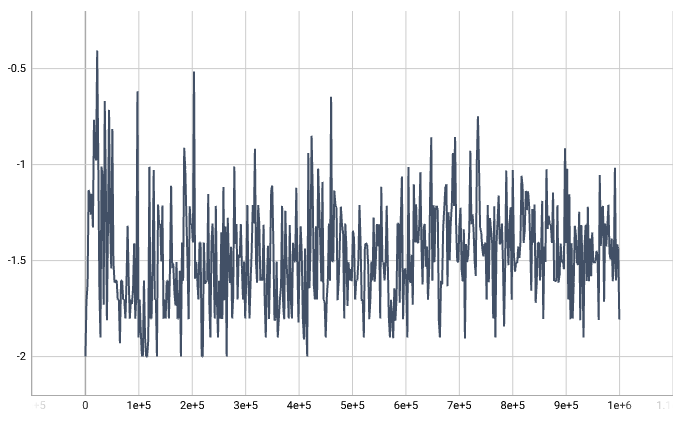
\includegraphics[width=\linewidth]{graphs/test_attacker_agent_return_mean_independent.PNG}
    \caption{Attacker episode returns}
  \end{subfigure}
  \begin{subfigure}[b]{0.49\linewidth}
    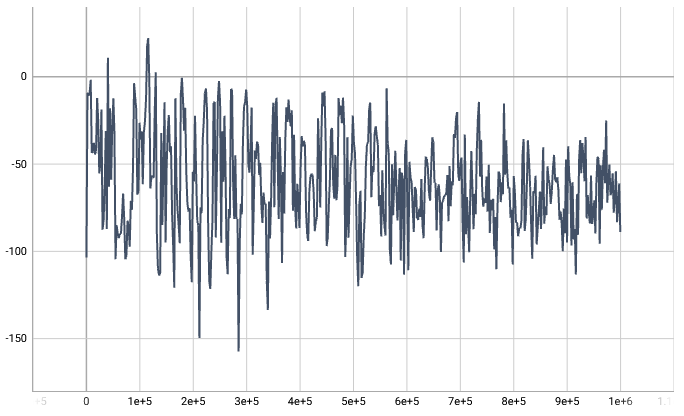
\includegraphics[width=\linewidth]{graphs/test_identifier_agent_return_mean_independent.PNG}
    \caption{Identifier episode returns}
  \end{subfigure}
  \caption{Learning with independent reward structure}
  \label{fig:coffee}
\end{figure}

\subsubsection{Agents with normal reward structure}
\begin{figure}[h!]
  \centering
  \begin{subfigure}[b]{0.49\linewidth}
    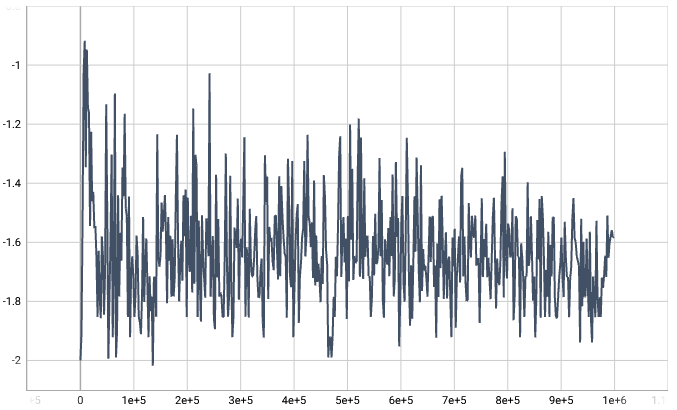
\includegraphics[width=\linewidth]{graphs/test_attacker_agent_return_mean_notindependent.PNG}
    \caption{Attacker episode returns}
  \end{subfigure}
  \begin{subfigure}[b]{0.49\linewidth}
    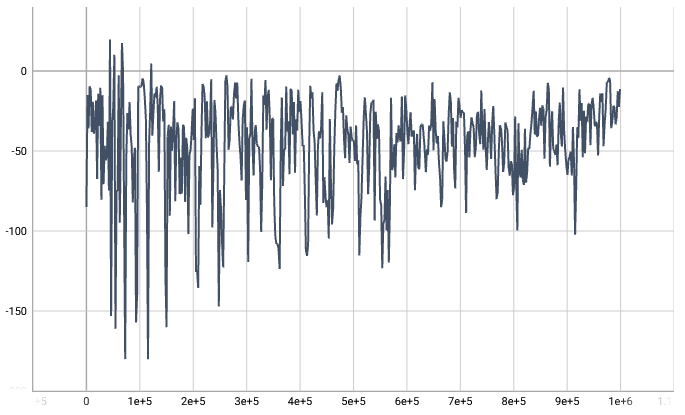
\includegraphics[width=\linewidth]{graphs/test_identifier_agent_return_mean_notindependent.PNG}
    \caption{Identifier episode returns}
  \end{subfigure}
  \caption{Learning with normal reward structures}
  \label{fig:coffee}
\end{figure}
\paragraph{Experiment setup.}
In this simulation, we set up an experiment with the expected settings of reward structures. The attacker receives positive rewards when consensus is breached and negative when its controlled malicious nodes were correctly identified, while the identifier receives positive rewards for correct attribution and negative for consensus violation.  
\paragraph{Results.} Similar to the previous experiment, the agents were not able to find an ideal policy within the given training periods and showed the comparable oscillation pattern. It was a likely result as the previous experiment demonstrated that the agents were not able to solve independent tasks with simpler reward structures.

\subsection{Discussion}\label{sec:discussion}
As the attribution game is not an environment designed as the playground for MARL algorithms, numerous of its peculiarities could be troublesome to the convergence of an ideal equilibrium or the mastery of a reward-yielding strategies. Having shown the limited progress we obtained in experiments, we would like to discuss the potential reasons and corresponding remedies for the hurdles during training.
\paragraph{The curse of dimensionality and variable order.} As action space and observation space in the attribution game consist of numerous messages received by several nodes with each message containing various contents, the total number of dimensions grows combinatorially. In addition to high number of dimensionalities in action and observation space, variable order also leads agent to unlikely encounter positive strategies through randomized exploration, causing it to remain stuck at suboptimal states.\\
{\bf{Remedy}}: A potential remedy would be to consider context-conditioned policies, which are classes policies conditioned by a probabilistic variable sampled from a latent encoder that takes the sequence of past observations as input \cite{DBLP:journals/corr/abs-1903-08254} \cite{DBLP:journals/corr/abs-1802-07245}. As the stochastic context variable is used to condition policies to choose actions, it provides structured exploration for the agents to potentially escape suboptimal states.

\paragraph{Sparse reward signals.}As the reward conditions in attribution game are when the attacker successfully breached consensus or when the identifier have correctly attributed more than $f+1$ malicious nodes, the agents barely receive any other useful reinforcements in most timesteps, leading to great difficulty of finding ideal policies. \\
{\bf{Remedy}}: A potential remedy would be to manually craft more reward conditions, for example, when the attacker has learnt to send valid certificates, or when the attacker has caused a honest node to deviate from the proper block. These conditions can give agents more reinforcement signals to guide them towards the direction of policies that yield high expected returns.


\paragraph{The ``Lazy Agent'' problem.} The ``lazy agent'' problem occurs in the fully cooperative games where the environment gives shared reward signals to all agents. Due to the difficulty of achieving credit assignment, agents with positive behaviors and those with idle actions would be encouraged equally, leading to suboptimal collective performance. Although the attribution game is not a cooperative game, the malicious nodes under the control of the attacker are in a fully cooperative relationship, receiving a shared reward signal without credit decomposition. It might cause the inability of the attacker agent to find an ideal collective strategy, particularly when the number of malicious nodes grows. \\ {\bf{Remedy}}: A potential remedy would be to allow malicious nodes as fully decentralized actors without considering the attacker as a centralized controller, this might further complicate the game dynamics of the attribution problem. Another remedy would be to allow a certain degree of decentralized agency in malicious nodes and to have the attacker learn how to conduct value decomposition mechanism to properly incentivize the individual malicious nodes \cite{DBLP:journals/corr/SunehagLGCZJLSL17}. 




%\section{Conclusion}\label{sec:conclusion}
%- Challenges you faced
%- What are your learnings?
%- Future work/insights on what should be done next
\section{Future work}\label{sec:future}
For the future work, we are still very driven to solve the two proposed questions on what is the minimal number of monitored transcripts to deter attacks and on what is the dynamics of different attack strategies under different priorities. Despite limited for now, both approaches, game theory and MARL, remain great potential to answer them. 

% {\color{george} summarize the approaches of game theory} \\
We find the potential of game theoretic analysis limited by the combinatorial complexity of strategies in terms of number of transcripts available to the identifier. The problem would be almost impossible to formulate for more complicated settings than discussed in this project. Therefore, we consider it only a theoretic basics for more advanced techniques like MARL. However, the insights which such analysis provide is valuable and would be necessary for any alternative approaches.

For MARL, the learning algorithm has great potential of improvements: as discussed in Section 6.5, a better candidate would be to have context-conditioned policy for structured exploration, manual reward structure to avoid sparse reinforcement signals, and value decomposition for better credit assignments to the malicious nodes. Future work on MARL would be to improve the learning performance along these mentioned directions.

\bibliography{citation.bib}
\bibliographystyle{ieeetr}

\end{document}